\begin{enumerate}[\bf 1.]
	\item 치환함수 $S:\set{0,1}^3\to\set{0,1}^3$가 다음과 같이 정의되었다고 하자.
	\begin{table}[h!]\centering\setstretch{1.5}
		\begin{tabular}{|c||c|c|c|c|c|c|c|c|}
			\hline
			$x$ & 0(000) & 1(001) & 2(010) & 3(011) & 4(100) & 5(101) & 6(110) & 7(111) \\
			\hline
			$S[x]$ & 0 & 2 & 4 & 6 & 5 & 7 & 3 & 1 \\
			\hline
		\end{tabular}
	\end{table}
	\begin{enumerate}[(a)]
		\item 입력차분이 $\alpha=4$일 때, 출력차분이 $\beta$가 될 확률 $P[\alpha\to\beta]$의 최댓값과 그 때의 $\beta$를 구하면?
		\item 입력 마스크가 $a=6(110)$이고 출력 마스크가 $b=2(010)$일 때 \[
		NS(a,b)=\set{x\mid a\cdot x=b\cdot S[x]}
		\]의 원소의 개수는? 임이의 입력 $x$에 대하여 $a\cdot x=b\cdot S[x]$가 만족될 확률은?
	\end{enumerate}
	\begin{proof}[\sol]
		\ \begin{enumerate}[(a)]
			\item 
			\ \begin{table}[h!]\centering\setstretch{1.25}
				\begin{tabular}{cc|cc|c}
					\toprule[1.2pt]
					$x$ & $x\oplus 100$ & $S[x]$ & $S[x\oplus 100]$ & $\beta=S[x]\oplus S[x\oplus 100]$\\ \hline
					000 & 100 & 000 & 101 & 101 \\
					001 & 101 & 010 & 111 & 101 \\
					010 & 110 & 100 & 011 & 111 \\
					011 & 111 & 110 & 001 & 111 \\
					100 & 000 & 101 & 000 & 101 \\
					101 & 001 & 111 & 010 & 101 \\
					110 & 010 & 011 & 100 & 111 \\
					111 & 011 & 001 & 110 & 111 \\
					\bottomrule[1.2pt]
				\end{tabular}
			\end{table}\\ 따라서 $\beta\in\set{(101)_2, (111)_2}=\set{5,7}$ 일 때, $$
			P[100\to 101]=\frac{1}{2}=P[100\to 111]$$ 이다.
			\newpage
			\item Let $x=(x_2x_1x_0)_2$ and $S[x]=(y_2y_1y_0)_2$. Consider $a=(110)_2$ and $b=(010)_2$: 
%			\begin{figure}[h!]\centering
%				\begin{tikzpicture}[>=Latex, node distance=1cm and 0cm]
%					% Nodes for inputs x
%					\node (x2) {\textcolor{red}{$x_2$}};
%					\node (x1) [right=of x2] {\textcolor{red}{$x_1$}};
%					\node (x0) [right=of x1] {$x_0$};
%					
%					% S-Box
%					\node (S) [draw, minimum size=1.5cm, below=of x1, xshift=0cm] {S};
%					
%					% Nodes for outputs y
%					\node (y2) [below=of S, xshift=-.5cm] {$y_2$};
%					\node (y1) [right=of y2] {\textcolor{red}{$y_1$}};
%					\node (y0) [right=of y1] {{$y_0$}};
%					
%					% Arrows from x to S
%					\draw[->, red, line width=1.25] (x2) -- (x2|-S.north);
%					\draw[->, red, line width=1.25] (x1) -- (x1|-S.north);
%					\draw[->] (x0) -- (x0|-S.north);
%					
%					% Arrows from S to y (ensuring alignment with x_i nodes)
%					\draw[->] (S.south-|x2) -- (x2|-y2.north);
%					\draw[->, red, line width=1.25] (S.south-|x1) -- (x1|-y1.north);
%					\draw[->] (S.south-|x0) -- (x0|-y0.north);
%				\end{tikzpicture}
%			\end{figure}\ \\	
			\begin{table}[h!]\centering\renewcommand{\arraystretch}{1}
				\begin{tabular}{ccc|ccc|cc}
					\toprule[1.2pt]
					\textcolor{red}{$[x_2]$} & \textcolor{red}{$[x_1]$} & $x_0$ & $y_2$ & \textcolor{red}{$[y_1]$} & {$y_0$} & $a\cdot x=b\cdot y$ & \\
					\hline
					0 & 0 & 0 & 0 & 0 & 0 & $0=0$ & \textcolor{green}{\checkmark}\\
					0 & 0 & 1 & 0 & 1 & 0 & $0=1$ & \textcolor{red}{\xmark}\\
					0 & 1 & 0 & 1 & 0 & 0 & $1=0$ & \textcolor{red}{\xmark}\\
					0 & 1 & 1 & 1 & 1 & 0 & $1=1$ & \textcolor{green}{\checkmark}\\
					1 & 0 & 0 & 1 & 0 & 1 & $1=0$ & \textcolor{red}{\xmark}\\
					1 & 0 & 1 & 1 & 1 & 1 & $1=1$ & \textcolor{green}{\checkmark}\\
					1 & 1 & 0 & 0 & 1 & 1 & $0=1$ & \textcolor{red}{\xmark}\\
					1 & 1 & 1 & 0 & 0 & 1 & $0=0$ & \textcolor{green}{\checkmark}\\
					\bottomrule[1.2pt]
				\end{tabular}
			\end{table}\\ 따라서 집합 $NS(a,b)$의 원소의 개수는 4이고, 임이의 입력 $x$에 대하여 $a\cdot x=b\cdot S[x]$가 만족될 확률은 $\frac{4}{8}=\frac{1}{2}$이다.
		\end{enumerate}
	\end{proof}
	\item 표본공간(sample space) $\set{0,1}$인 독립확률변수(independent random variable) $X_1,X_2,X_3$가 \[
	P[X_1=0]=P[X_2=0]=P[X_3=0]=\frac{3}{4}
	\]를 만족할 때, Piling-up lemma를 이용하여 확률 $P[X_1\oplus X_2\oplus X_3=0]$을 구하면?
	\begin{proof}[\sol]
		\ \begin{tcolorbox}[colback=white]
			\textbf{Theorem} (Piling-Up Lemma)\textbf{.}\quad
			Let $X_i\in\set{0,1}$ is independent binary random variables. Then \[
			\Pr\left[\bigoplus_{i=1}^nX_i=0\right]=\frac{1}{2}+2^{n-1}\prod_{i=1}^n\left(p_i-\frac{1}{2}\right)
			\] where $p_i=\Pr[X_i=0]$ and $\bigoplus$ denotes the XOR operation.
		\end{tcolorbox}
		Thus, \begin{align*}
			P[X_1\oplus X_2\oplus X_3=0] &= \frac{1}{2}+2^{3-1}\left(\frac{3}{4}-\frac{1}{2}\right)\left(\frac{3}{4}-\frac{1}{2}\right)\left(\frac{3}{4}-\frac{1}{2}\right)\\
			&=\frac{1}{2}+4\cdot\left(\frac{1}{4}\right)^3\\
			&=\frac{1}{2}+\frac{1}{16}=\frac{9}{16}.
		\end{align*}
	\end{proof}
%	\item 이중 암호화를 사용한 블록암호의 MITM(Meet-in-the-Middle) 공격에 대하여 다음 물음에 답하라.
%	\begin{itemize}
%		\item 사용한 블록암호: $C=E(P,key)$
%		\item 입출력 크기: 64비트
%		\item 암호키: 56비트
%		\item 암호 알고리즘 $C=E(E(P,key1),key2)$
%	\end{itemize}
%	\begin{enumerate}[(a)]
%		\item 한개의 (평문, 암호문) 쌍으로부터 얻어지는 후보키의 개수를 예상하면? 이때, 암호키는 후보키에 반드시 포함되는가?
%		\item 높은 확률로 암호키 후보 한개만 남도록 하려면 (평문, 암호문) 쌍이 몇 개 필요한가?
%		\item MITM 공격에 필요한 메모리의 크기는?
%	\end{enumerate}
%	\newpage
%	\item 다음 그림과 같은 4라운드 암호 알고리즘 $Enc:\set{0,1}^{32}\to\set{0,1}^{32}$을 생각하자.
%	\begin{itemize}
%		\item 암호화 $C=Enc(P,key)$
%		\item 입출력 크기: 32비트
%		\item 암호키: 20바이트 ($rk_0,rk_1,\dots,rk_4$는 각각 4바이트)
%	\end{itemize}
%	\begin{figure}[h!]\centering
%		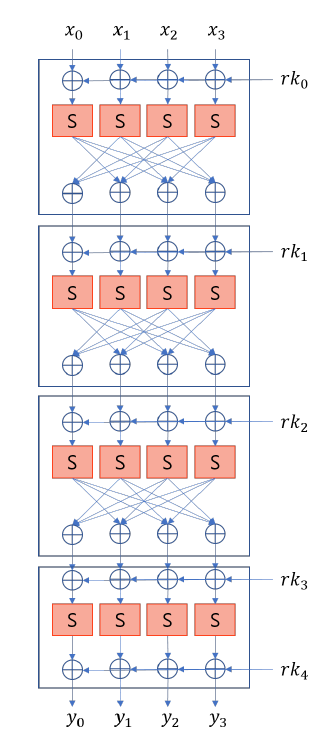
\includegraphics[scale=.5]{final1}
%	\end{figure}
%	\begin{center}
%		$S:\set{0,1}^8\to\set{0,1}^8$의 차분 확률 $P[\alpha\to\beta]$ \\
%		\vfill
%		\begin{tabular}{c|c|c}
%			\hline
%			\multicolumn{3}{c}{차분확률 $P[\alpha\to\beta]$} \\ \hline
%			$P[\texttt{0x01}\to\texttt{0x01}]=0.0$ & $P[\texttt{0x0F}\to\texttt{0x01}]=0.0$ & $P[\texttt{0xFF}\to\texttt{0x01}]=0.063$ \\
%			$P[\texttt{0x01}\to\texttt{0x02}]=0.016$ & $P[\texttt{0x0F}\to\texttt{0x02}]=0.016$ & $P[\texttt{0xFF}\to\texttt{0x02}]=0.016$ \\
%			$P[\texttt{0x01}\to\texttt{0x0F}]=0.25$ & $P[\texttt{0x0F}\to\texttt{0x0F}]=0.0$ & $P[\texttt{0xFF}\to\texttt{0x0F}]=0.0$ \\
%			$P[\texttt{0x01}\to\texttt{0x10}]=0.0$ & $P[\texttt{0x0F}\to\texttt{0x10}]=0.0$ & $P[\texttt{0xFF}\to\texttt{0x10}]=0.0$ \\
%			$P[\texttt{0x01}\to\texttt{0xFF}]=0.25$ & $P[\texttt{0x0F}\to\texttt{0xFF}]=0.25$ & $P[\texttt{0xFF}\to\texttt{0xFF}]=0.016$ \\
%			$\vdots$ & $\vdots$ & $\vdots$ \\ \hline
%		\end{tabular}
%	\end{center}
%	\newpage
%	\begin{enumerate}[(a)]
%		\item 주어진 $S$의 차분확률표를 이용하여 차분공격에 필요한 차분특성을 구성하고 차분확률을 계산하면?
%		\item (a)에서 구성한 차분특성으로 차분공격을 구성하자. 차분공격에 필요한 선택평문, 암호문 쌍을 충분히 수집했다고 가정하고, 이를 이용한 공격 알고리즘을 설명해라. 이 때, $rk_4$ 중 한바이트를 얻기 위해 예측해야 하는 정보는 몇 비트이며 공격에 필요한 계산량은 얼마인가?
%	\end{enumerate}
%	\begin{proof}[\sol]
%		\ \begin{enumerate}[(a)]
%			\item 
%		\end{enumerate}
%	\end{proof}
\end{enumerate}